\documentclass[10pt]{beamer}
\usetheme[
%%% option passed to the outer theme
%    progressstyle=fixedCircCnt,   % fixedCircCnt, movingCircCnt (moving is deault)
]{Feather}
  
% If you want to change the colors of the various elements in the theme, edit and uncomment the following lines

% Change the bar colors:
%\setbeamercolor{Feather}{fg=red!20,bg=red}

% Change the color of the structural elements:
%\setbeamercolor{structure}{fg=red}

% Change the frame title text color:
%\setbeamercolor{frametitle}{fg=blue}

% Change the normal text color background:
%\setbeamercolor{normal text}{fg=black,bg=gray!10}

%-------------------------------------------------------
% INCLUDE PACKAGES
%-------------------------------------------------------

\usepackage[utf8]{inputenc}
\usepackage[italian]{babel}
\usepackage{helvet}
\usepackage{listings}
\usepackage{xcolor}
\usepackage{graphicx}
\usepackage{multirow}

%-------------------------------------------------------
% DEFFINING AND REDEFINING COMMANDS
%-------------------------------------------------------

% colored hyperlinks
\newcommand{\chref}[2]{
  \href{#1}{{\usebeamercolor[bg]{Feather}#2}}
}

%-------------------------------------------------------
% INFORMATION IN THE TITLE PAGE
%-------------------------------------------------------

\title[Performance Modeling of Computer Systems and Networks] % [] is optional - is placed on the bottom of the sidebar on every slide
{ % is placed on the title page
      \textbf{Performance Modeling of Computer Systems and Networks}
}

\subtitle[ - Project 2018-2019]
{
      \textbf{Project 2018-2019}
}

\author[Andrea Graziani - 0273395]
{      Andrea Graziani - 0273395 \\
      {}
}

\institute[]
{
      Universit`a degli Studi di Roma “Tor Vergata” \\
      FACOLTA' DI INGEGNERIA \\
      Corso di Laurea Magistrale in Ingegneria Informatica
  
  %there must be an empty line above this line - otherwise some unwanted space is added between the university and the country (I do not know why;( )
}

\date{\today}

% ----------------------------------------------------------------------------------------- %
% Usato per personalizzare l'ambiente 'listings'...
% ----------------------------------------------------------------------------------------- %
\lstset{
language=C,
basicstyle=\tiny\ttfamily,			
keywordstyle=\color{blue},
commentstyle=\color{gray},			
stringstyle=\color{black},			
%numbers=left,						
%numberstyle=\tiny,					
%stepnumber=1,						
breaklines=true						
}

%-------------------------------------------------------
% THE BODY OF THE PRESENTATION
%-------------------------------------------------------

\begin{document}

%-------------------------------------------------------
% THE TITLEPAGE
%-------------------------------------------------------

{\1% % this is the name of the PDF file for the background
\begin{frame}[plain,noframenumbering] % the plain option removes the header from the title page, noframenumbering removes the numbering of this frame only
  \titlepage % call the title page information from above
\end{frame}}






\section{System State}
\subsection{Mathematical variables}
% ************************************************************************** %
\begin{frame}[fragile]{Mathematical variables}{Specification Model}

\begin{itemize}


\item Mathematical notation and variables used in our specification model:

\begin{table}[h!]
    \centering
    \small
    \begin{tabular}{l}
      $c \in \lbrace 1,2 \rbrace = C$ \\
      $x \in \lbrace cloudlet,cloud,global \rbrace = X$ \\
      $\tau \in (t_0, t)$ \\       
    \end{tabular}
\end{table}

\begin{table}[h!]
    \centering
    \small
    \begin{tabular}{l}
      $n_x^{(c)}(\tau)$  \\
      $d_x^{(c)}(\tau)$  \\
      $s_{x,i}^{(c)}$  \\
      $i_{cloudlet}^{(2)}(\tau)$ \\
          
    \end{tabular}
\end{table}

\item There are several constrains and relations among these variables.
\begin{itemize}
\item Some of which depend on chosen access control algorithm.
\end{itemize}

\end{itemize}

\end{frame}

% ************************************************************************** %
\subsection{System State}
\begin{frame}[fragile]{System State}{Specification Model}

\begin{equation}
\omega(\tau) = (\omega_{cloudlet}(\tau),\omega_{cloud}(\tau))
\end{equation}

Where:

\begin{equation}
\begin{array} {rcl} 
\omega_{cloudlet}(\tau) & = & (n_{cloudlet}^{(1)}(\tau),n_{cloudlet}^{(2)}(\tau)) \\
\omega_{cloud}(\tau) & = & (n_{cloud}^{(1)}(\tau),n_{cloud}^{(2)}(\tau)) \\
\end{array}
\end{equation}

Thus:

\begin{equation}
\begin{array} {rcl} 
\omega(\tau) = ((n_{cloudlet}^{(1)}(\tau),n_{cloudlet}^{(2)}(\tau)),(n_{cloud}^{(1)}(\tau),n_{cloud}^{(2)}(\tau))
\end{array}
\end{equation}
\end{frame}

% ************************************************************************** %
\subsection{System assumptions}
\begin{frame}[fragile]{System assumptions}{Specification Model}
\begin{itemize}
\item $n_x^{(c)}(0) = 0$ and $d_x^{(c)}(0) = 0$, $\forall c \in C, \forall x \in X $
\begin{itemize}
\item Initial system status is \textit{idle}. 
\end{itemize}



\item First event must be either a class 1 or class 2 job arrival.

\item Our stopping criteria: $\tau^*$ beyond which no new jobs can arrive.
\begin{itemize}
\item Terminal state is idle.
\item System keep on working until all jobs have been completely served. 
\end{itemize}


\end{itemize}
\end{frame}



% ************************************************************************** %
\subsection{Events (Algorithm 1)}
\begin{frame}[fragile]{Events (Algorithm 1)}{Specification Model}

\begin{figure}
\centering
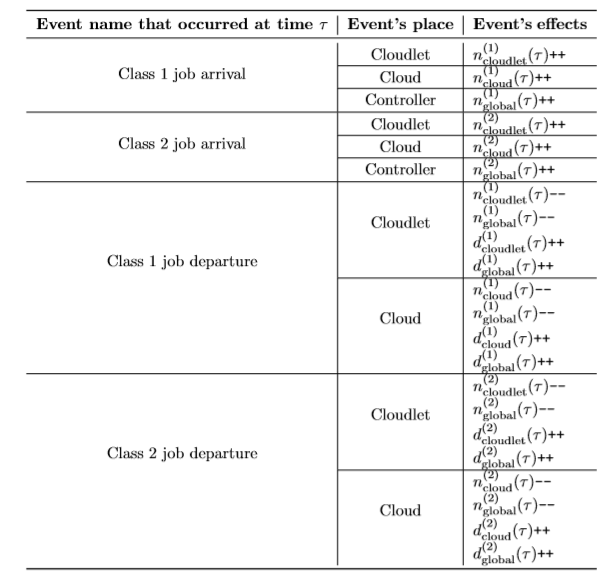
\includegraphics[width=\textwidth, height=200px]{./images/EventsSpec.png}
\label{fig:Concorrente}
\end{figure}

\end{frame}

% ************************************************************************** %
\subsection{Events (Algorithm 2)}
\begin{frame}[fragile]{Events (Algorithm 2)}{Specification Model}

\begin{equation}
\begin{array} {rcl} 

n_{cloudlet}^{(1)}(\tau) & \neq & N \\\\

n_{cloudlet}^{(1)}(\tau) + n_{cloudlet}^{(2)}(\tau) & > & S \\\\

n_{cloudlet}^{(2)} & \geqslant & 0

\end{array}
\end{equation}

\begin{itemize}
\item $n_{cloudlet}^{(1)}(\tau)$ is incremented by one.
\item $n_{cloudlet}^{(2)}(\tau)$ is decremented by one.
\item class 2 job arrival on cloud node event is scheduled (considering a set-up time)
\end{itemize}


\end{frame}

\section{Computational Model}
% ************************************************************************** %
\subsection{Next-event simulation logic}
\begin{frame}[fragile]{Class Diagrams 1}{Computational Model}
\begin{figure}
\centering
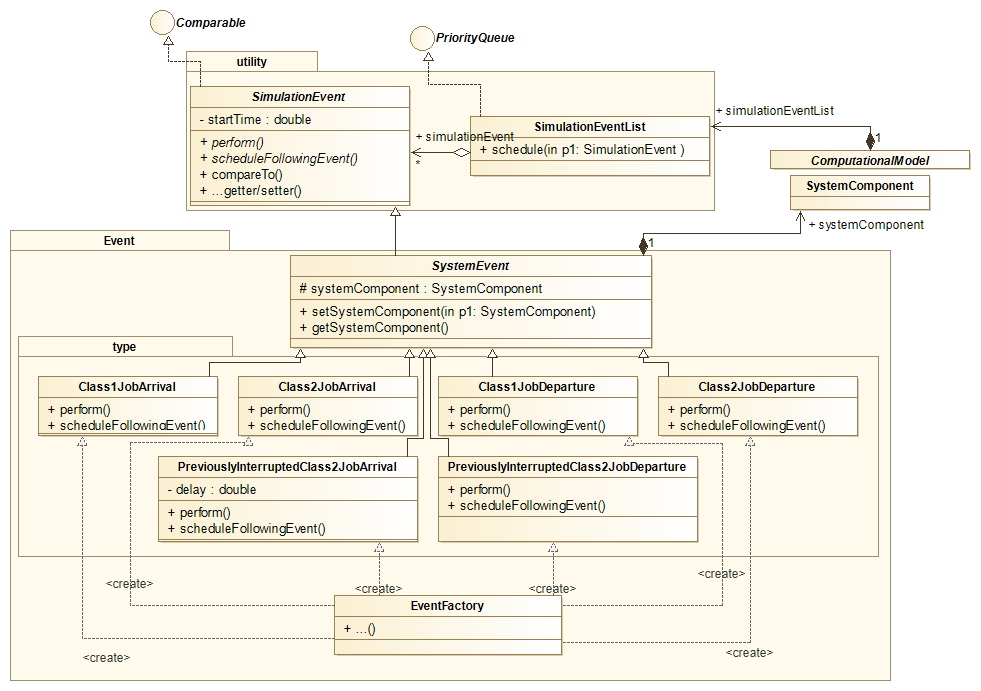
\includegraphics[width=\textwidth]{./images/ClassDiagramEvent.png}
\label{fig:Concorrente}
\end{figure}


\end{frame}

% ************************************************************************** %
\subsection{Next-event simulation logic}
\begin{frame}[fragile]{Class Diagrams 2}{Computational Model}
\begin{figure}
\centering
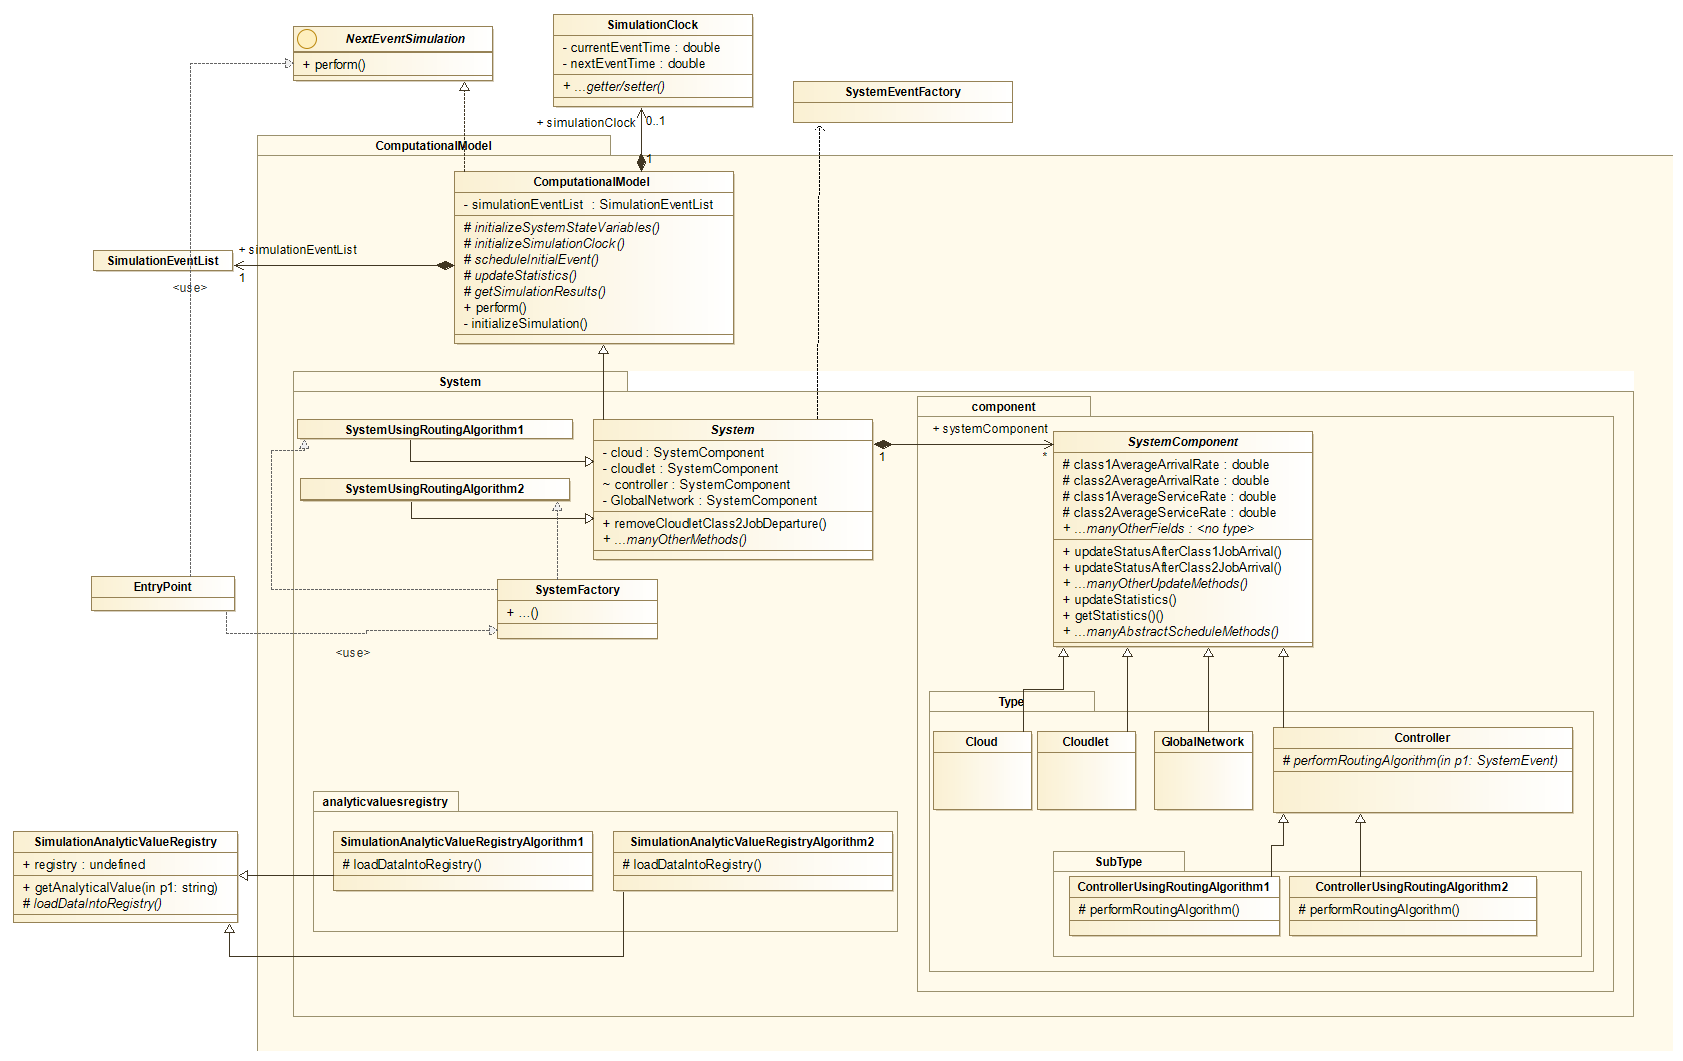
\includegraphics[width=\textwidth]{./images/ClassDiagram.png}
\label{fig:Concorrente}
\end{figure}


\end{frame}


% ************************************************************************** %
\subsection{Next-event simulation logic}
\begin{frame}[fragile]{Next-event simulation logic}{Computational Model}

\begin{lstlisting}[frame=lines, caption={Snippet of \texttt{perform} method}, label={code:perform}]
public void perform() {

   initializeSimulation();
   
   while (!this.simulationEventList.isEmpty()) {

      SimulationEvent actualEvent = this.simulationEventList.poll();

      if (actualEvent != null) {

          SimulationClock.getInstance().setCurrentEventTime(actualEvent.getStartTime());

          actualEvent.perform();
          actualEvent.scheduleFollowingEvent();

          SimulationEvent nextEvent = this.simulationEventList.peek();

          if (nextEvent != null)
              SimulationClock.getInstance().setNextEventTime(nextEvent.getStartTime());
      }
      updateStatistics();
   }
...
\end{lstlisting}
\end{frame}

% ************************************************************************** %
\subsection{Routing algorithm 1}
\begin{frame}[fragile]{Routing algorithm 1}{Computational Model}

\begin{lstlisting}
protected void performRoutingAlgorithm(SystemEvent event) {

   int n1 = this.system.getNumberOfClass1JobOnCloudlet();
   int n2 = this.system.getNumberOfClass2JobOnCloudlet();

   if ((n1 + n2) == this.system.getThreshold())
      this.system.scheduleEventOnCloud(event, 0);
   else
      this.system.scheduleEventOnCloudlet(event, 0);
}
\end{lstlisting}
\end{frame}

% ************************************************************************** %
\subsection{Routing algorithm 2}
\begin{frame}[fragile]{Routing algorithm 2}{Computational Model}

\begin{lstlisting}
protected void performRoutingAlgorithm(SystemEvent event) {

    int n1 = this.system.getNumberOfClass1JobOnCloudlet();
    int n2 = this.system.getNumberOfClass2JobOnCloudlet();

        if (event instanceof Class1JobArrival) {

            if (n1 == this.system.getThreshold())
                this.system.scheduleEventOnCloud(event, 0);
            else if (n1 + n2 < this.system.getThreshold())
                this.system.scheduleEventOnCloudlet(event, 0);
            else if (n2 > 0) {

                double runningCloudletTimeOfInterruptedJob = this.system.removeCloudletClass2JobDeparture();

                this.system.scheduleEventOnCloudlet(event, 0);

                double setupTime = RandomNumberGenerator.getInstance().getExponential(5, 0.8);

                this.system.scheduleEventOnCloud(SystemEventFactory.buildPreviouslyInterruptedClass2JobArrival(setupTime + runningCloudletTimeOfInterruptedJob), setupTime);

                this.numberOfInterruptedClass2Jobs++;

            } else
                this.system.scheduleEventOnCloudlet(event, 0);


        } else {

            ...
        }
    }
\end{lstlisting}
\end{frame}


\section{Statistics Results}

% ----------------------------------------------------------------------------------------- %
\begin{frame}[fragile]{Statistics Results}{Il processo client}

\vspace*{20px}
Do \textbf{steady-state} statistics exist?


\end{frame}

\begin{frame}[fragile]{Statistics Results}{Il processo client}
\begin{figure}
\centering
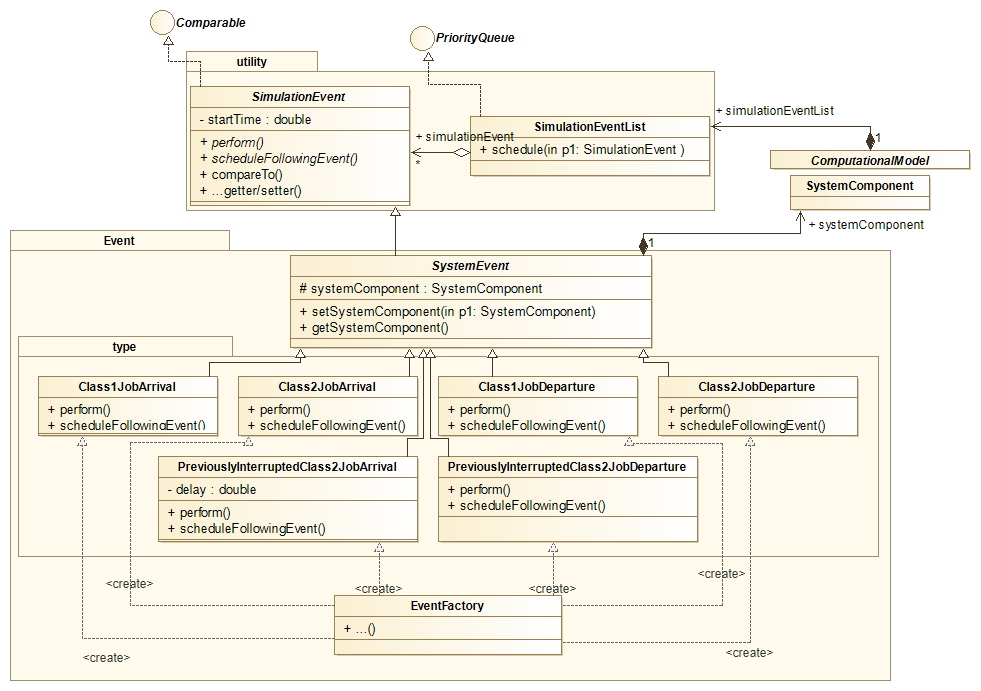
\includegraphics[width=\textwidth]{./images/ClassDiagramEvent.png}
\caption{Class 1 Jobs Service Time}
\label{fig:Concorrente}
\end{figure}


\end{frame}


% ----------------------------------------------------------------------------------------- %
\begin{frame}[fragile]{Statistics Results}{Il processo client}

\begin{block}{Steady-state system statistics}
\textbf{Steady-state system statistics} are those statistics, if they exist, that are produced by simulating the operation of a \textbf{stationary} discrete-event system for an effectively \textbf{infinite} length of time.

In many systems, a steady state is not achieved until some time after the system is started or initiated. This initial situation is often identified as a transient state, start-up or warm-up period.

If a system is in a steady state, then the recently observed behavior of the system will continue into the future.

if the variables (called state variables) which define the behavior of the system or the process are unchanging in time.

\end{block}
\end{frame}

% ----------------------------------------------------------------------------------------- %
\begin{frame}[fragile]{Statistics Results}{}

\begin{figure}
\centering
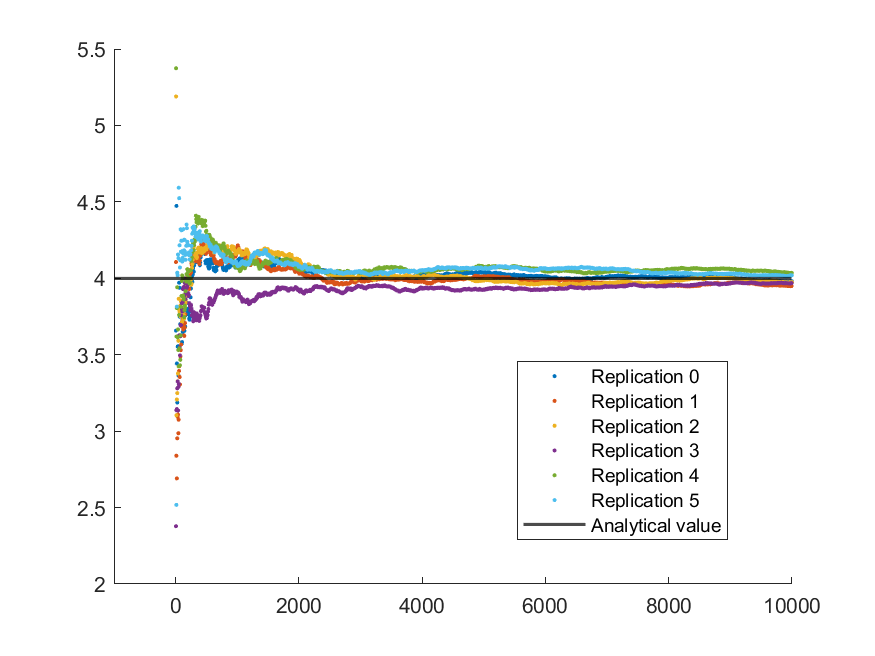
\includegraphics[width=\textwidth]{./images/ScatterPlotCloud_Class1JobsServiceTime.png}
\caption{Class 1 Jobs Service Time}
\label{fig:Concorrente}
\end{figure}


\end{frame}





{\1
\begin{frame}[plain,noframenumbering]
  \finalpage{Grazie per l'attenzione!}
\end{frame}}


\end{document}